% Native long-division carry changes subsequent integer grid placement.
\documentclass[border=2pt]{standalone}
\usepackage{tikz}
\begin{document}
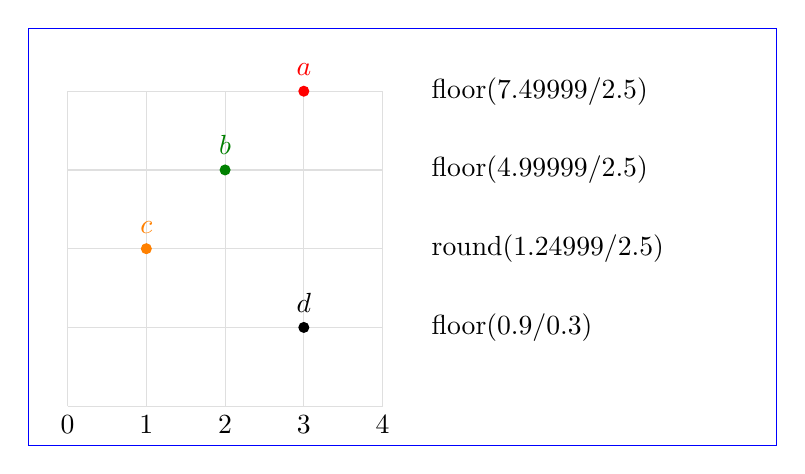
\begin{tikzpicture}
  \draw[blue] (-.5,-.5) rectangle (9,4.8);
  \draw[gray!25] (0,0) grid (4,4);
  \foreach \x in {0,1,2,3,4} \node[below] at (\x,0) {$\x$};
  \node[anchor=west] at (4.5,4) {floor$(7.49999/2.5)$};
  \node[anchor=west] at (4.5,3) {floor$(4.99999/2.5)$};
  \node[anchor=west] at (4.5,2) {round$(1.24999/2.5)$};
  \node[anchor=west] at (4.5,1) {floor$(0.9/0.3)$};
  \fill[red] ({floor(7.49999/2.5)},4) circle (2pt) node[above=2pt] {$a$};
  \fill[green!50!black] ({floor(4.99999/2.5)},3) circle (2pt) node[above=2pt] {$b$};
  \fill[orange] ({round(1.24999/2.5)},2) circle (2pt) node[above=2pt] {$c$};
  \fill[black] ({floor(0.9/0.3)},1) circle (2pt) node[above=2pt] {$d$};
\end{tikzpicture}
\end{document}
